\documentclass{article}
\usepackage{graphicx}
\usepackage{geometry}
\usepackage{hyperref}
\usepackage{booktabs}
\usepackage{subcaption}
\usepackage{amsmath}

\geometry{
    a4paper,
    margin=0.6in
}

\hypersetup{
    colorlinks=true,
    linkcolor=blue,
    filecolor=magenta,
    urlcolor=cyan,
}

\title{SNN Atan $\alpha$ Convergence Analysis\\vs CNN Baseline (MNIST)}
\author{ByzFL SNN Benchmark}
\date{\today}

\begin{document}

\maketitle

\section{Overview}
This document presents training convergence plots comparing Spiking Neural Network (SNN) models with different ArcTangent surrogate gradient scaling factors $\alpha \in \{1.0, 1.25, 1.5, 2.0, 3.0\}$ and the CNN baseline.

\textbf{Experimental settings:}
\begin{itemize}
    \item \textbf{Dataset:} MNIST
    \item \textbf{Aggregator:} GeometricMedian (with NNM + ARC pre-aggregation)
    \item \textbf{Attack:} Optimal A Little Is Enough
    \item \textbf{Honest clients:} $n_h = 10$, Byzantine: $f \in \{0, 3, 5\}$
    \item \textbf{Data heterogeneity:} $\gamma \in \{1.0, 0.33, 0.0\}$ (IID $\to$ extreme non-IID)
    \item \textbf{Seeds:} 5 seeds (mean $\pm$ std shading)
\end{itemize}


\newpage
\section{Test Accuracy over Training Steps}
Each panel shows test accuracy as a function of training step for SNN with different $\alpha$ values (solid colored lines) and the CNN baseline (dashed black).

\begin{figure}[htbp]
    \centering
    \begin{subfigure}[b]{0.32\textwidth}
        \centering
        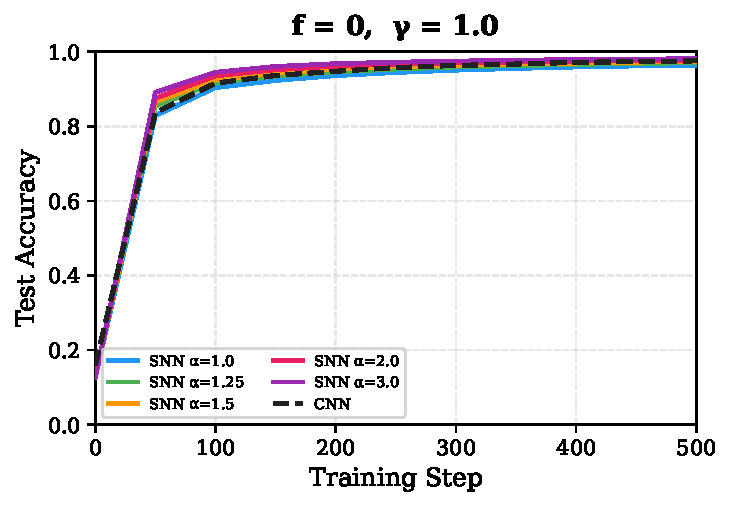
\includegraphics[width=\textwidth]{../plots/snn/alpha_convergence_grid/test_accuracy_f0_gamma1_0.pdf}
        \caption{$f=0$, $\gamma=1.0$}
        \label{fig:acc_f0_g1_0}
    \end{subfigure}
    \hfill
    \begin{subfigure}[b]{0.32\textwidth}
        \centering
        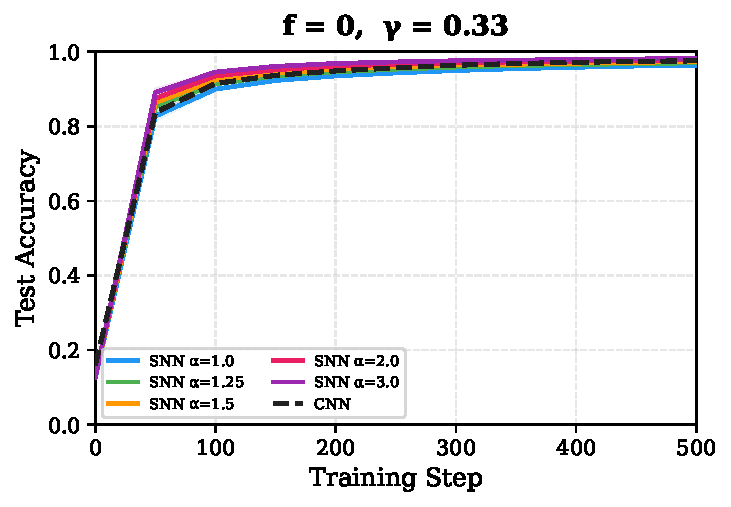
\includegraphics[width=\textwidth]{../plots/snn/alpha_convergence_grid/test_accuracy_f0_gamma0_33.pdf}
        \caption{$f=0$, $\gamma=0.33$}
        \label{fig:acc_f0_g0_33}
    \end{subfigure}
    \hfill
    \begin{subfigure}[b]{0.32\textwidth}
        \centering
        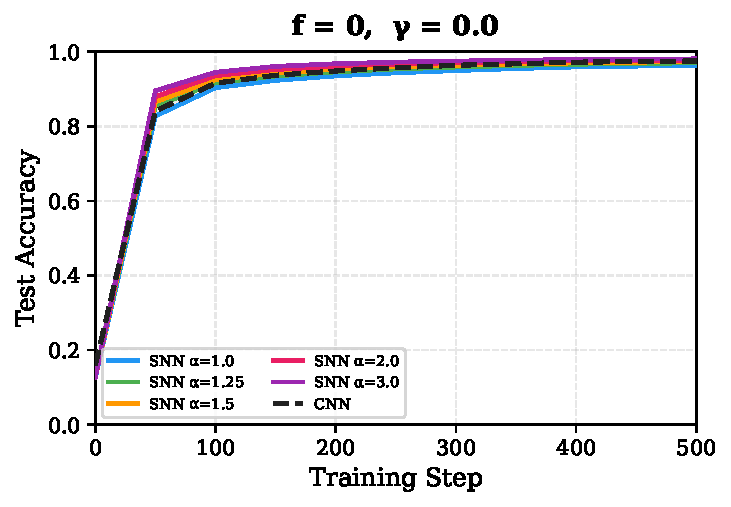
\includegraphics[width=\textwidth]{../plots/snn/alpha_convergence_grid/test_accuracy_f0_gamma0_0.pdf}
        \caption{$f=0$, $\gamma=0.0$}
        \label{fig:acc_f0_g0_0}
    \end{subfigure}

    \vspace{0.3cm}

    \begin{subfigure}[b]{0.32\textwidth}
        \centering
        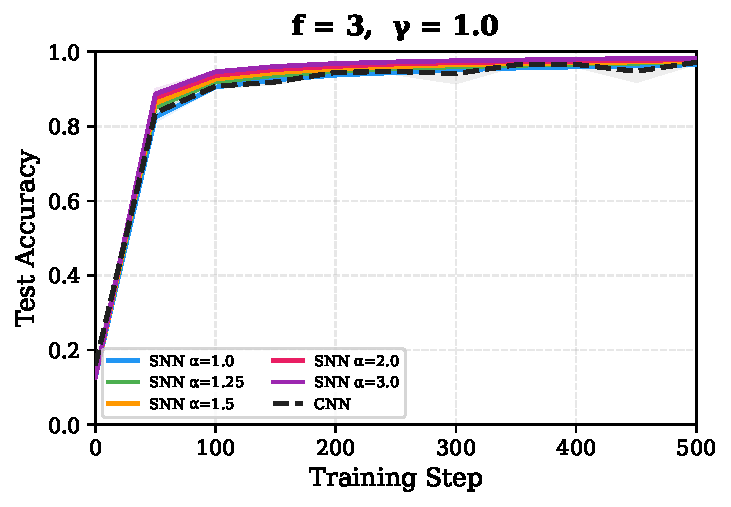
\includegraphics[width=\textwidth]{../plots/snn/alpha_convergence_grid/test_accuracy_f3_gamma1_0.pdf}
        \caption{$f=3$, $\gamma=1.0$}
        \label{fig:acc_f3_g1_0}
    \end{subfigure}
    \hfill
    \begin{subfigure}[b]{0.32\textwidth}
        \centering
        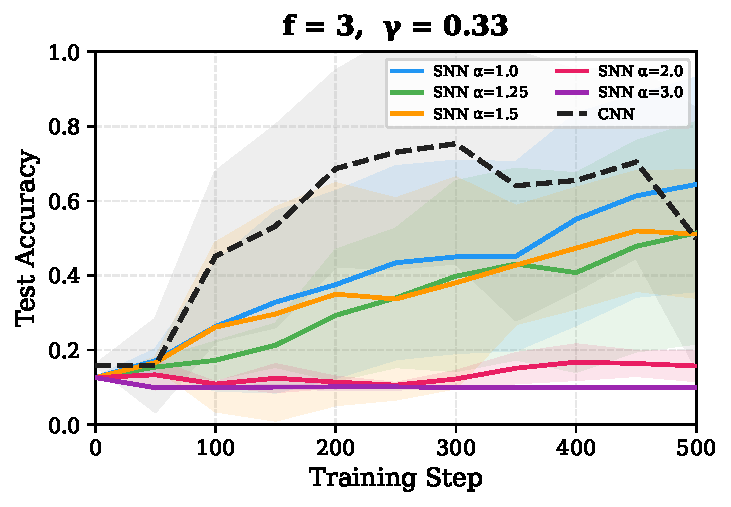
\includegraphics[width=\textwidth]{../plots/snn/alpha_convergence_grid/test_accuracy_f3_gamma0_33.pdf}
        \caption{$f=3$, $\gamma=0.33$}
        \label{fig:acc_f3_g0_33}
    \end{subfigure}
    \hfill
    \begin{subfigure}[b]{0.32\textwidth}
        \centering
        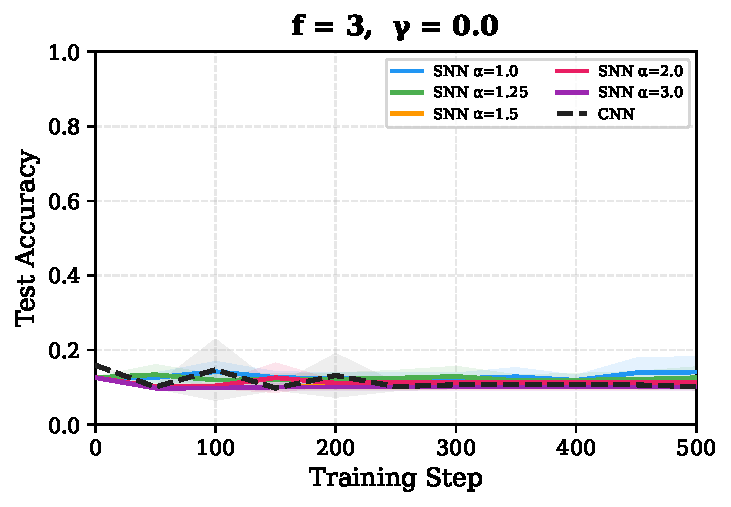
\includegraphics[width=\textwidth]{../plots/snn/alpha_convergence_grid/test_accuracy_f3_gamma0_0.pdf}
        \caption{$f=3$, $\gamma=0.0$}
        \label{fig:acc_f3_g0_0}
    \end{subfigure}

    \vspace{0.3cm}

    \begin{subfigure}[b]{0.32\textwidth}
        \centering
        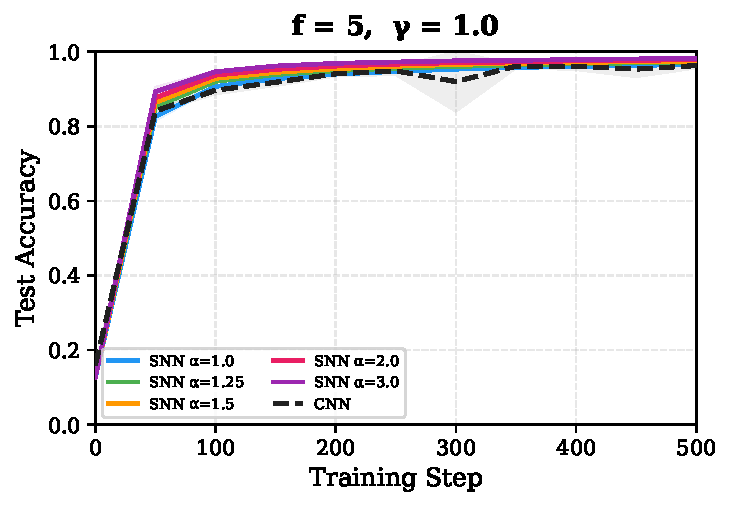
\includegraphics[width=\textwidth]{../plots/snn/alpha_convergence_grid/test_accuracy_f5_gamma1_0.pdf}
        \caption{$f=5$, $\gamma=1.0$}
        \label{fig:acc_f5_g1_0}
    \end{subfigure}
    \hfill
    \begin{subfigure}[b]{0.32\textwidth}
        \centering
        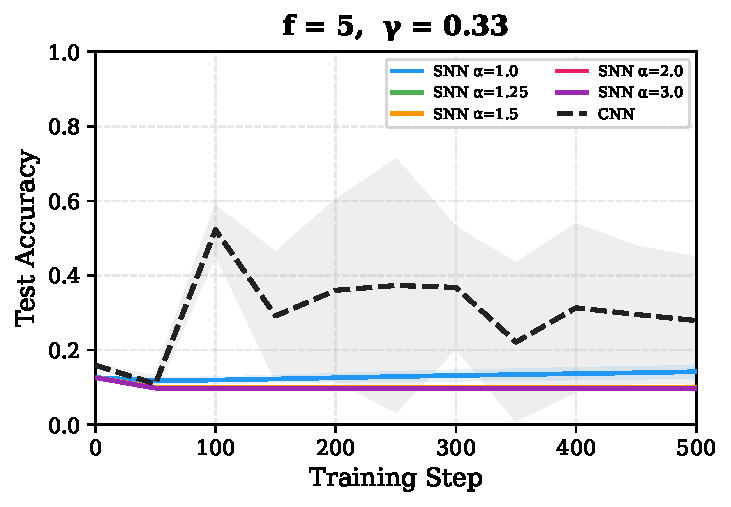
\includegraphics[width=\textwidth]{../plots/snn/alpha_convergence_grid/test_accuracy_f5_gamma0_33.pdf}
        \caption{$f=5$, $\gamma=0.33$}
        \label{fig:acc_f5_g0_33}
    \end{subfigure}
    \hfill
    \begin{subfigure}[b]{0.32\textwidth}
        \centering
        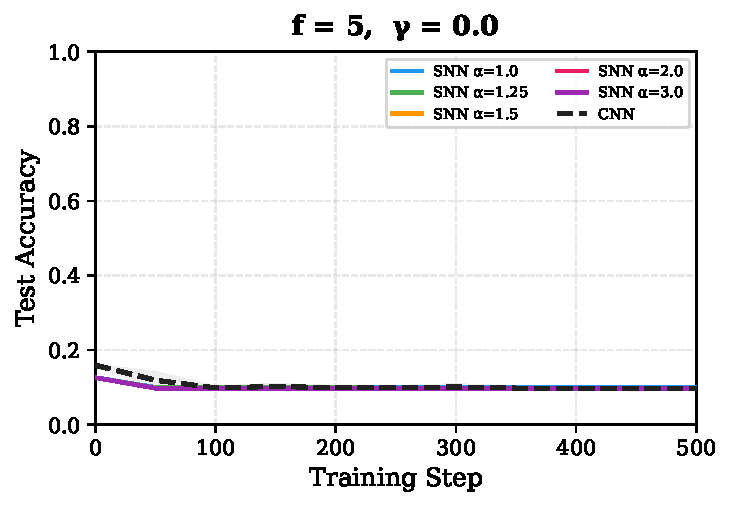
\includegraphics[width=\textwidth]{../plots/snn/alpha_convergence_grid/test_accuracy_f5_gamma0_0.pdf}
        \caption{$f=5$, $\gamma=0.0$}
        \label{fig:acc_f5_g0_0}
    \end{subfigure}

    \caption{Test Accuracy convergence: SNN ($\alpha \in \{1.0, 1.25, 1.5, 2.0, 3.0\}$) vs CNN baseline. Rows: increasing Byzantine fraction ($f$). Columns: decreasing data IID-ness ($\gamma$).}
    \label{fig:test_accuracy_grid}
\end{figure}


\newpage
\section{Train Loss over Training Steps (SNN Only)}
Train loss for SNN models only. CNN loss is omitted because the loss functions are not comparable (SNN uses rate-coded cross-entropy, CNN uses NLL loss).

\begin{figure}[htbp]
    \centering
    \begin{subfigure}[b]{0.32\textwidth}
        \centering
        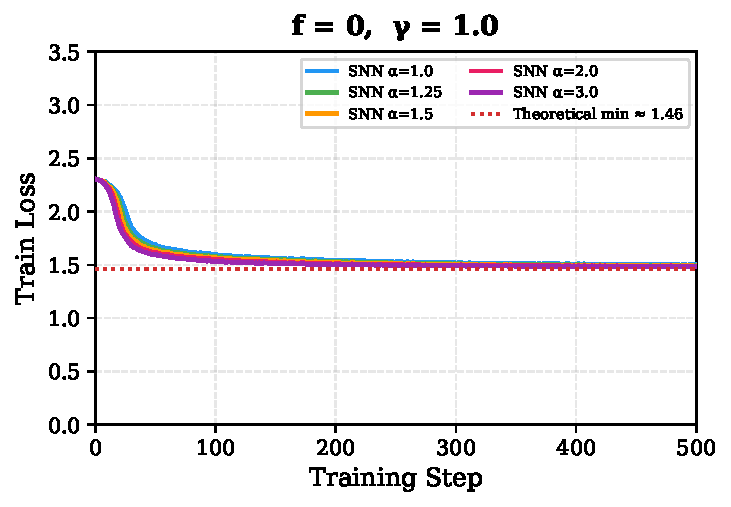
\includegraphics[width=\textwidth]{../plots/snn/alpha_convergence_grid/train_loss_f0_gamma1_0.pdf}
        \caption{$f=0$, $\gamma=1.0$}
        \label{fig:loss_f0_g1_0}
    \end{subfigure}
    \hfill
    \begin{subfigure}[b]{0.32\textwidth}
        \centering
        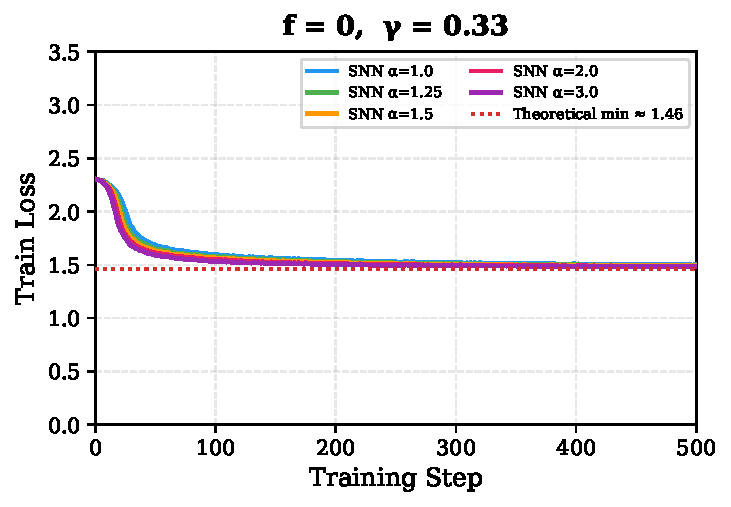
\includegraphics[width=\textwidth]{../plots/snn/alpha_convergence_grid/train_loss_f0_gamma0_33.pdf}
        \caption{$f=0$, $\gamma=0.33$}
        \label{fig:loss_f0_g0_33}
    \end{subfigure}
    \hfill
    \begin{subfigure}[b]{0.32\textwidth}
        \centering
        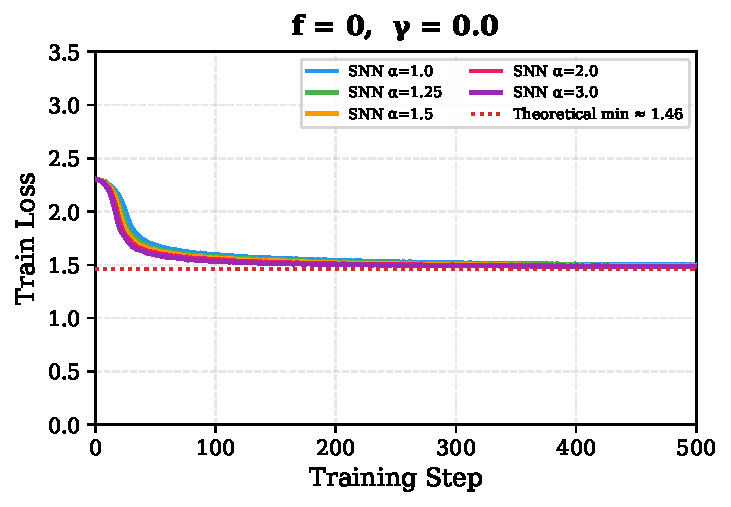
\includegraphics[width=\textwidth]{../plots/snn/alpha_convergence_grid/train_loss_f0_gamma0_0.pdf}
        \caption{$f=0$, $\gamma=0.0$}
        \label{fig:loss_f0_g0_0}
    \end{subfigure}

    \vspace{0.3cm}

    \begin{subfigure}[b]{0.32\textwidth}
        \centering
        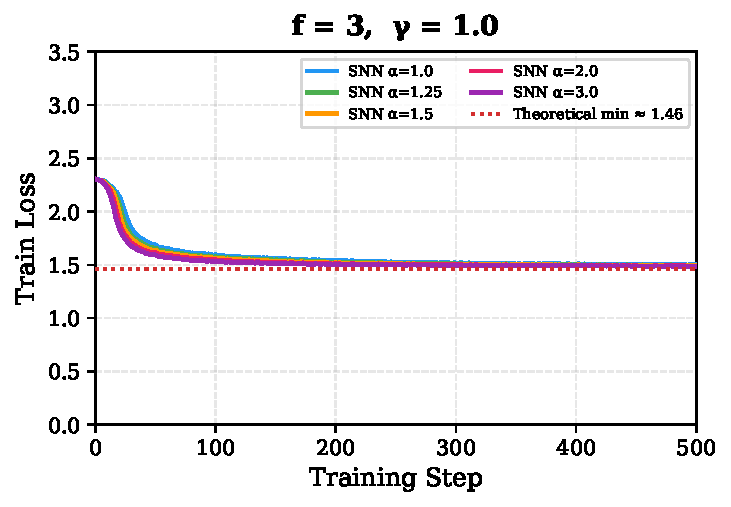
\includegraphics[width=\textwidth]{../plots/snn/alpha_convergence_grid/train_loss_f3_gamma1_0.pdf}
        \caption{$f=3$, $\gamma=1.0$}
        \label{fig:loss_f3_g1_0}
    \end{subfigure}
    \hfill
    \begin{subfigure}[b]{0.32\textwidth}
        \centering
        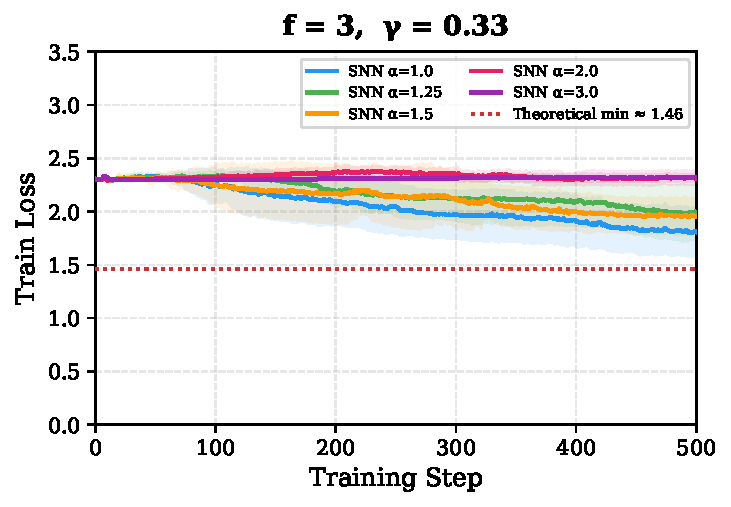
\includegraphics[width=\textwidth]{../plots/snn/alpha_convergence_grid/train_loss_f3_gamma0_33.pdf}
        \caption{$f=3$, $\gamma=0.33$}
        \label{fig:loss_f3_g0_33}
    \end{subfigure}
    \hfill
    \begin{subfigure}[b]{0.32\textwidth}
        \centering
        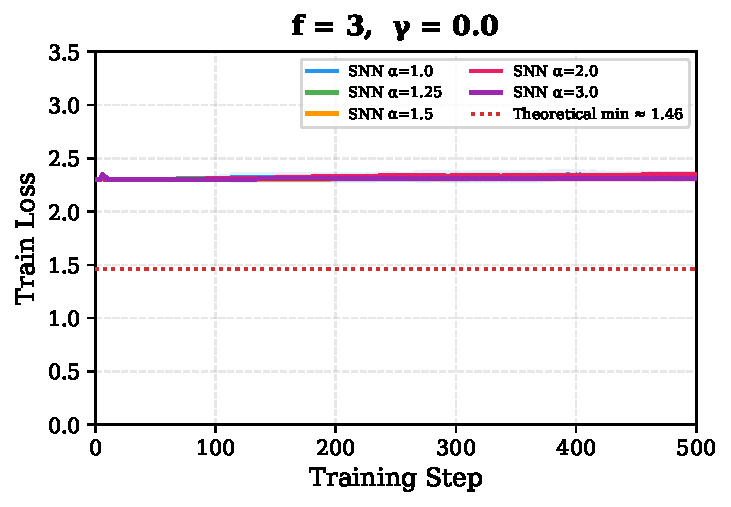
\includegraphics[width=\textwidth]{../plots/snn/alpha_convergence_grid/train_loss_f3_gamma0_0.pdf}
        \caption{$f=3$, $\gamma=0.0$}
        \label{fig:loss_f3_g0_0}
    \end{subfigure}

    \vspace{0.3cm}

    \begin{subfigure}[b]{0.32\textwidth}
        \centering
        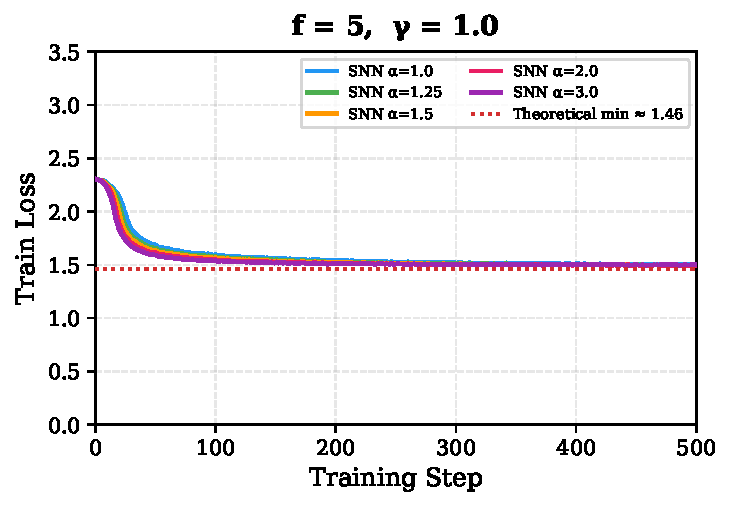
\includegraphics[width=\textwidth]{../plots/snn/alpha_convergence_grid/train_loss_f5_gamma1_0.pdf}
        \caption{$f=5$, $\gamma=1.0$}
        \label{fig:loss_f5_g1_0}
    \end{subfigure}
    \hfill
    \begin{subfigure}[b]{0.32\textwidth}
        \centering
        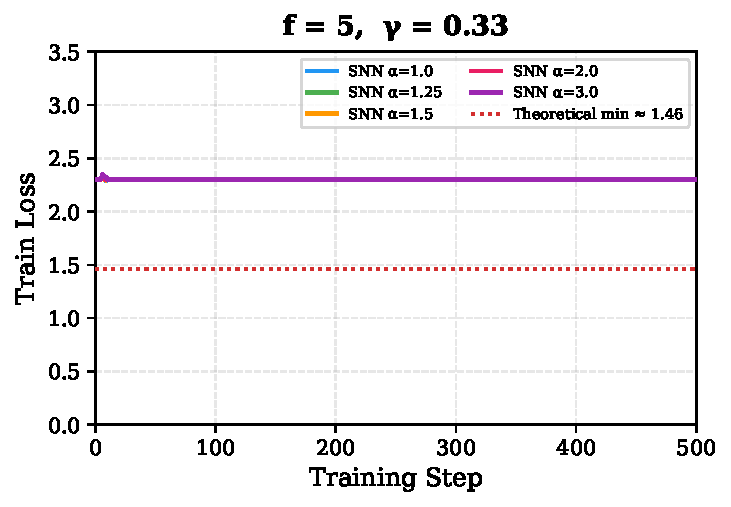
\includegraphics[width=\textwidth]{../plots/snn/alpha_convergence_grid/train_loss_f5_gamma0_33.pdf}
        \caption{$f=5$, $\gamma=0.33$}
        \label{fig:loss_f5_g0_33}
    \end{subfigure}
    \hfill
    \begin{subfigure}[b]{0.32\textwidth}
        \centering
        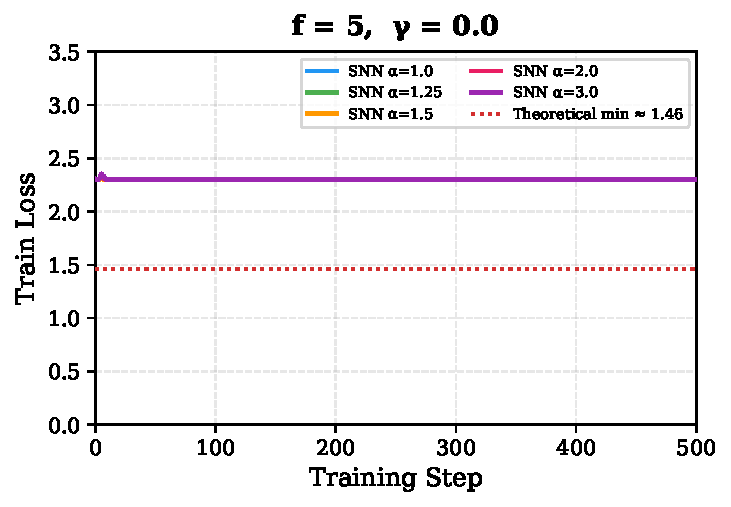
\includegraphics[width=\textwidth]{../plots/snn/alpha_convergence_grid/train_loss_f5_gamma0_0.pdf}
        \caption{$f=5$, $\gamma=0.0$}
        \label{fig:loss_f5_g0_0}
    \end{subfigure}

    \caption{Train Loss convergence for SNN only ($\alpha \in \{1.0, 1.25, 1.5, 2.0, 3.0\}$). CNN is excluded because loss functions are not directly comparable.}
    \label{fig:train_loss_grid}
\end{figure}


\newpage
\section{Train Loss over Training Steps (CNN Only)}
Train loss for the CNN baseline. Shown separately from SNN because the loss functions differ (CNN uses NLL loss, SNN uses rate-coded cross-entropy).

\begin{figure}[htbp]
    \centering
    \begin{subfigure}[b]{0.32\textwidth}
        \centering
        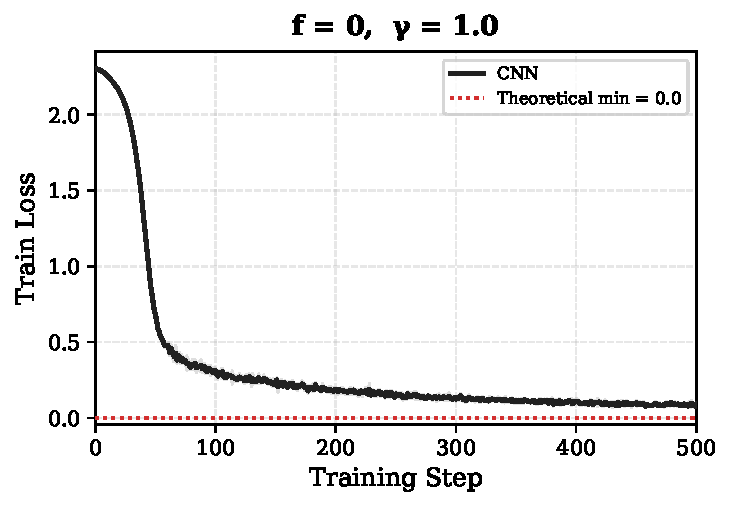
\includegraphics[width=\textwidth]{../plots/snn/alpha_convergence_grid/train_loss_cnn_f0_gamma1_0.pdf}
        \caption{$f=0$, $\gamma=1.0$}
        \label{fig:cnn_loss_f0_g1_0}
    \end{subfigure}
    \hfill
    \begin{subfigure}[b]{0.32\textwidth}
        \centering
        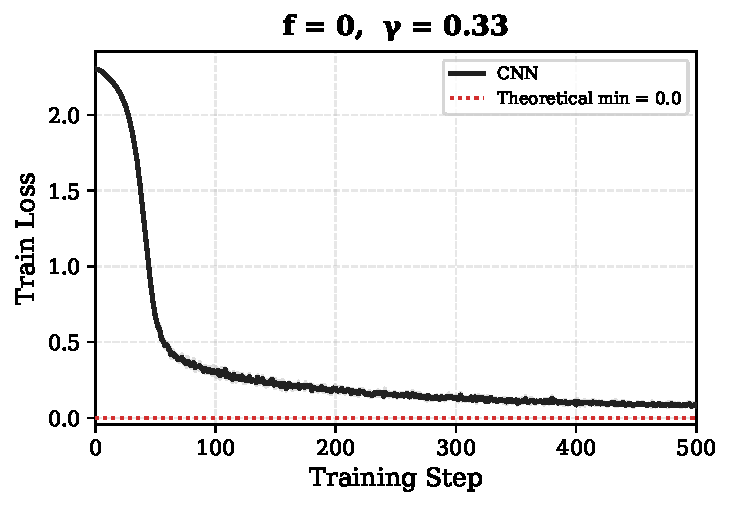
\includegraphics[width=\textwidth]{../plots/snn/alpha_convergence_grid/train_loss_cnn_f0_gamma0_33.pdf}
        \caption{$f=0$, $\gamma=0.33$}
        \label{fig:cnn_loss_f0_g0_33}
    \end{subfigure}
    \hfill
    \begin{subfigure}[b]{0.32\textwidth}
        \centering
        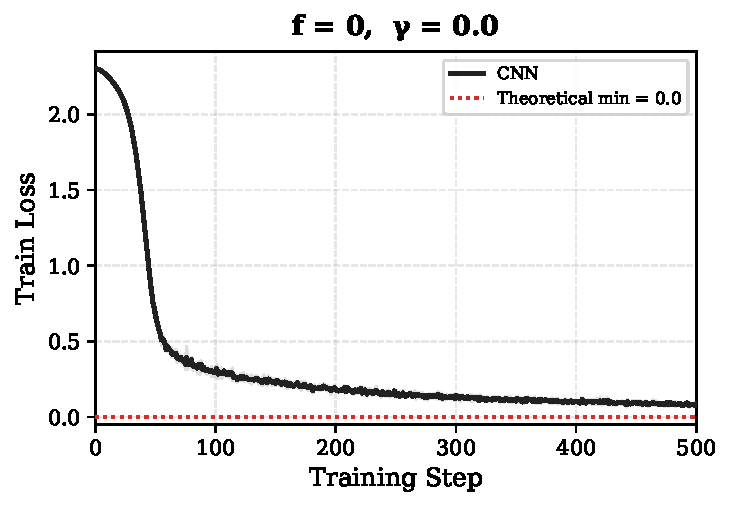
\includegraphics[width=\textwidth]{../plots/snn/alpha_convergence_grid/train_loss_cnn_f0_gamma0_0.pdf}
        \caption{$f=0$, $\gamma=0.0$}
        \label{fig:cnn_loss_f0_g0_0}
    \end{subfigure}

    \vspace{0.3cm}

    \begin{subfigure}[b]{0.32\textwidth}
        \centering
        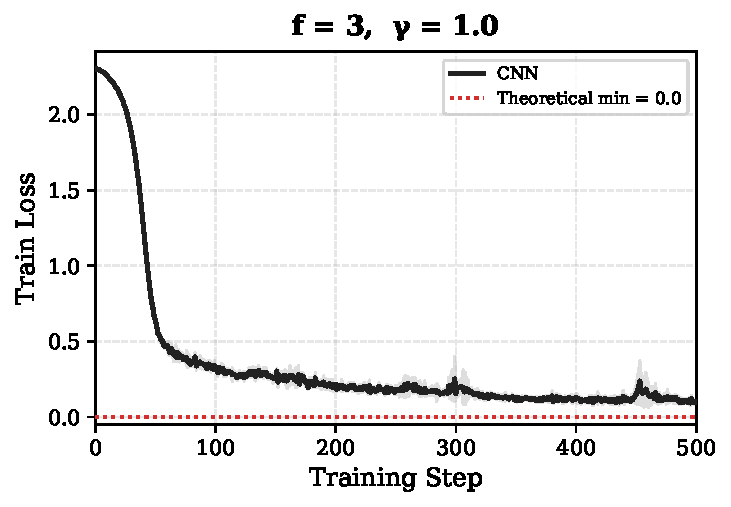
\includegraphics[width=\textwidth]{../plots/snn/alpha_convergence_grid/train_loss_cnn_f3_gamma1_0.pdf}
        \caption{$f=3$, $\gamma=1.0$}
        \label{fig:cnn_loss_f3_g1_0}
    \end{subfigure}
    \hfill
    \begin{subfigure}[b]{0.32\textwidth}
        \centering
        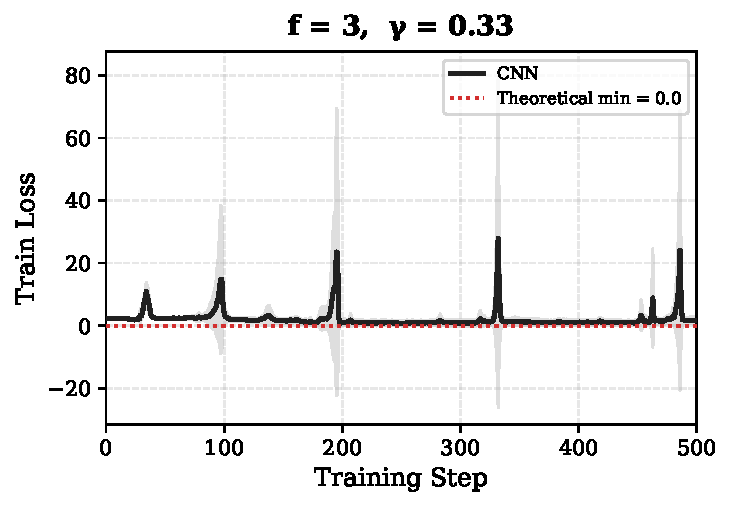
\includegraphics[width=\textwidth]{../plots/snn/alpha_convergence_grid/train_loss_cnn_f3_gamma0_33.pdf}
        \caption{$f=3$, $\gamma=0.33$}
        \label{fig:cnn_loss_f3_g0_33}
    \end{subfigure}
    \hfill
    \begin{subfigure}[b]{0.32\textwidth}
        \centering
        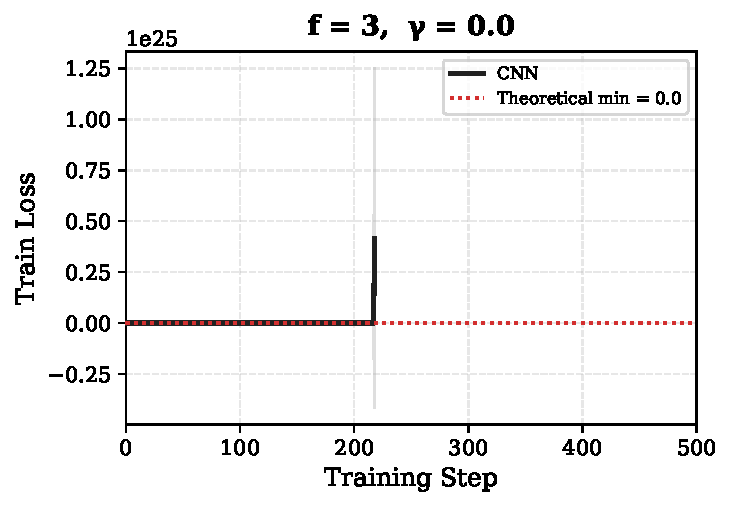
\includegraphics[width=\textwidth]{../plots/snn/alpha_convergence_grid/train_loss_cnn_f3_gamma0_0.pdf}
        \caption{$f=3$, $\gamma=0.0$}
        \label{fig:cnn_loss_f3_g0_0}
    \end{subfigure}

    \vspace{0.3cm}

    \begin{subfigure}[b]{0.32\textwidth}
        \centering
        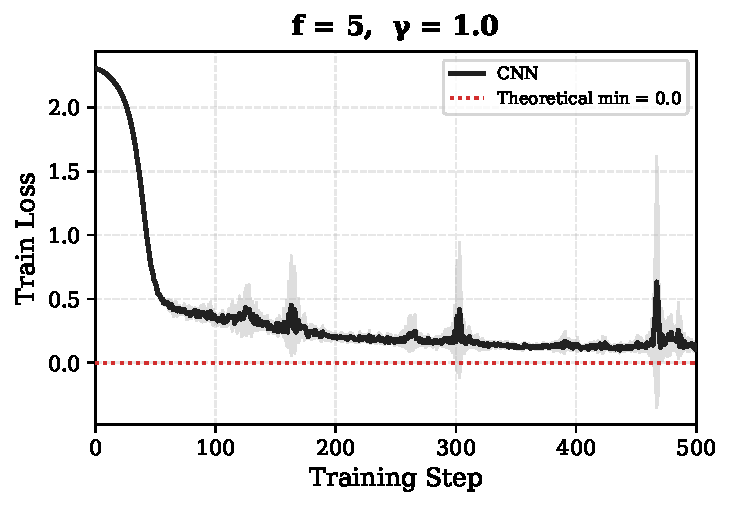
\includegraphics[width=\textwidth]{../plots/snn/alpha_convergence_grid/train_loss_cnn_f5_gamma1_0.pdf}
        \caption{$f=5$, $\gamma=1.0$}
        \label{fig:cnn_loss_f5_g1_0}
    \end{subfigure}
    \hfill
    \begin{subfigure}[b]{0.32\textwidth}
        \centering
        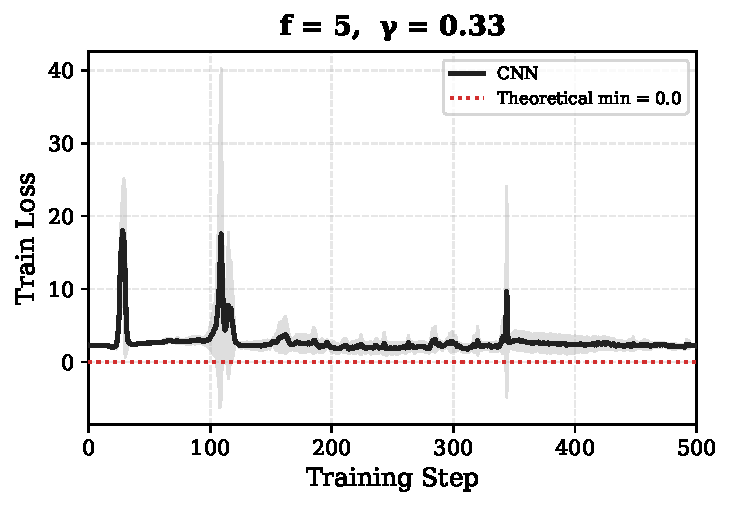
\includegraphics[width=\textwidth]{../plots/snn/alpha_convergence_grid/train_loss_cnn_f5_gamma0_33.pdf}
        \caption{$f=5$, $\gamma=0.33$}
        \label{fig:cnn_loss_f5_g0_33}
    \end{subfigure}
    \hfill
    \begin{subfigure}[b]{0.32\textwidth}
        \centering
        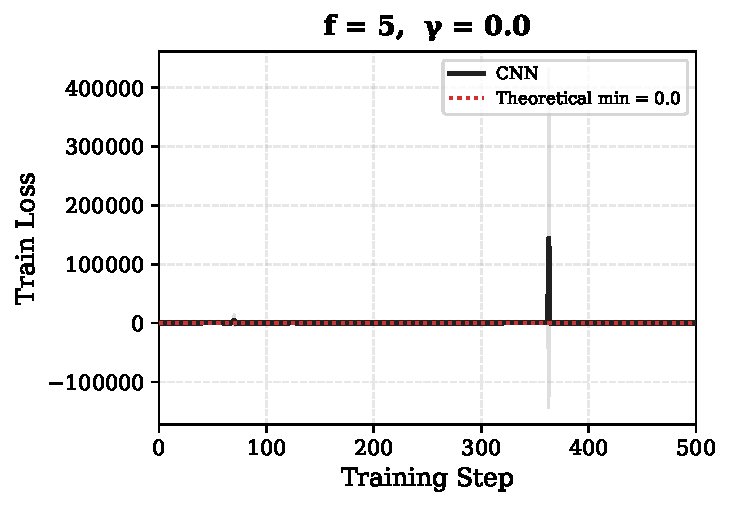
\includegraphics[width=\textwidth]{../plots/snn/alpha_convergence_grid/train_loss_cnn_f5_gamma0_0.pdf}
        \caption{$f=5$, $\gamma=0.0$}
        \label{fig:cnn_loss_f5_g0_0}
    \end{subfigure}

    \caption{Train Loss convergence for CNN baseline only (NLL Loss).}
    \label{fig:cnn_train_loss_grid}
\end{figure}

\section{Key Observations}
\begin{itemize}
    \item \textbf{Benign settings} ($f=0$, any $\gamma$): All $\alpha$ values converge similarly; higher $\alpha$ is slightly faster initially.
    \item \textbf{Moderate adversarial} ($f=3$, $\gamma=0.33$): $\alpha=1.0$ shows the most robustness, climbing to $\sim$65\% while $\alpha \geq 2.0$ collapse to random. CNN achieves higher but unstable accuracy.
    \item \textbf{IID under attack} ($f=3$ or $f=5$, $\gamma=1.0$): Surprisingly, higher $\alpha$ converges faster even under attack when data is IID.
    \item \textbf{Extreme adversarial} ($f=5$, $\gamma=0.0$): All models collapse to random accuracy.
    \item \textbf{Train loss stability}: SNN train loss is much smoother than CNN under Byzantine attack, suggesting intrinsic gradient stability of spiking networks.
\end{itemize}

\end{document}
